%%%%%%%%%%%%%%%%%%%%%%%%%%%%%%%%%%%%%%%%%%%%%%%%%%%%%%%%%%%%%%%%%%%%
%% I, the copyright holder of this work, release this work into the
%% public domain. This applies worldwide. In some countries this may
%% not be legally possible; if so: I grant anyone the right to use
%% this work for any purpose, without any conditions, unless such
%% conditions are required by law.
%%%%%%%%%%%%%%%%%%%%%%%%%%%%%%%%%%%%%%%%%%%%%%%%%%%%%%%%%%%%%%%%%%%%

\documentclass[
  digital, %% This option enables the default options for the
           %% digital version of a document. Replace with `printed`
           %% to enable the default options for the printed version
           %% of a document.
  table,   %% Causes the coloring of tables. Replace with `notable`
           %% to restore plain tables.
  lof,     %% Prints the List of Figures. Replace with `nolof` to
           %% hide the List of Figures.
  nolot,     %% Prints the List of Tables. Replace with `nolot` to
           %% hide the List of Tables.
  %% More options are listed in the user guide at
  %% <http://mirrors.ctan.org/macros/latex/contrib/fithesis/guide/mu/fi.pdf>.
]{fithesis3}
%% The following section sets up the locales used in the thesis.
\usepackage[resetfonts]{cmap} %% We need to load the T2A font encoding
\usepackage[T1,T2A]{fontenc}  %% to use the Cyrillic fonts with Russian texts.
\usepackage[
  main=english, %% By using `czech` or `slovak` as the main locale
                %% instead of `english`, you can typeset the thesis
                %% in either Czech or Slovak, respectively.
   czech %% The additional keys allow
]{babel}        %% foreign texts to be typeset as follows:
%%
%%   \begin{otherlanguage}{german}  ... \end{otherlanguage}
%%   \begin{otherlanguage}{russian} ... \end{otherlanguage}
%%   \begin{otherlanguage}{czech}   ... \end{otherlanguage}
%%   \begin{otherlanguage}{slovak}  ... \end{otherlanguage}
%%
%% For non-Latin scripts, it may be necessary to load additional
%% fonts:
\usepackage{paratype}
%%
%% The following section sets up the metadata of the thesis.
\thesissetup{
    date          = 2018/5/21,
    university    = mu,
    faculty       = fi,
    type          = mgr,
    author        = Václav Štěbra,
    gender        = m,
    advisor       = {doc. RNDr. Tomáš Pitner, Ph.D.},
    title         = {Komunikační portál založený na technologii WebRTC},
    TeXtitle      = {Komunikační portál založený na technologii WebRTC},
    keywords      = {online audio communication, onlide video communication, WebRTC, Javascript, HTML5},
    TeXkeywords   = {online audio communication, onlide video communication, WebRTC, Javascript, HTML5},
    abstract      = {The goal of this thesis is to build online meeting portal using the WebRTC technology. The main focus should be placed on scalability in multi-party calls and on great user experience.},
    thanks        = {These are the acknowledgements for my thesis, which can

                     span multiple paragraphs.},
    bib           = example.bib,
}
\usepackage{makeidx}      %% The `makeidx` package contains
\makeindex                %% helper commands for index typesetting.
%% These additional packages are used within the document:
\usepackage{paralist} %% Compact list environments
\usepackage{amsmath}  %% Mathematics
\usepackage{amsthm}
\usepackage{amsfonts}
\usepackage{url}      %% Hyperlinks
\usepackage{markdown} %% Lightweight markup
\usepackage{listings} %% Source code highlighting
\lstset{
  basicstyle      = \ttfamily,%
  identifierstyle = \color{black},%
  keywordstyle    = \color{blue},%
  keywordstyle    = {[2]\color{cyan}},%
  keywordstyle    = {[3]\color{olive}},%
  stringstyle     = \color{teal},%
  commentstyle    = \itshape\color{magenta}}
\usepackage{floatrow} %% Putting captions above tables
\floatsetup[table]{capposition=top}
\begin{document}
\chapter{Introduction}
\section{Motivation}
Online communication is becoming more and more important in today’s world. We use it every day to communicate with our family, friends and to communicate with our team members or customers in business environment. Home office or even remote work is becoming more and more popular among many businesses and their employees. Both sides can benefit from remote work. Employees are happy that they do not have to commute to work every day and can spent more time with their close ones. Businesses on the other hand can save some money as they do not have to keep permanent office space for the employee. With this trend comes great need for high quality and reliable way of communicating with the rest of the team.

This thesis is a follow up to the bachelor thesis WebRTC meeting portal  \cite{bachelorThesis} written in 2016. It was written as a proof of concept of “relatively” young and not yet widely used technology at that time called WebRTC\footnote{Web Real-Time Communication - https://webrtc.org/
}. Main goal was to build a usable meeting portal using newest web platform capabilities. The main ways of communicating using the portal are audio and video calls between two or more participants. It is also possible to exchange text messages and see the list of participants. Everything is secured so that only invited people can join the meeting.

The meeting portal is very simple and offers many opportunities for new functionality and improvements. It only allows authenticated users to participate in the conference call which on one hand provides better security for the meeting, but on the other hand it can drive some people away as they do not want to create account for yet another service. Especially when they want to use it one time. It was not built with scalability in mind and therefore only very small number of users is able the connect before the quality degrades. There is no possibility to mute the audio or screen share. This thesis elaborates on some of the mentioned shortcomings and introduces couple new features.

\section{Goal of the thesis}
The portal for which this thesis is a follow up was built as proof of concept to demonstrate the capabilities of the web platform regarding multimedia communication. Therefore, it has its shortcomings and usability problems as user experience was not its primary goal. Main disadvantage of the portal are high requirements on the user's bandwidth when participating in the multi-party conference call. That is not ideal when it could be used in business environment for communication between possibly large teams. Therefore, biggest focus and architecture goal of this thesis is to build the portal with a higher scalability in mind so that it can handle higher number of participants without big degradation of call quality.

Focus is also placed on better user experience. This includes features such as possibility to mute the microphone, disable camera feed or joining  the conference without the user account. Also, there will be possibility to share the screen.
 
File sharing is very useful feature that is often needed during meetings. It should be therefore possible to share files between the participants of the call. Also retrospective of the meeting can be quite useful to review what has been discussed on the meeting. After the meeting all users with an account who participated in the call will be able to access, view and download the recording of the call.

\section{Structure}
This work is divided into several chapters. First one serves as introduction of the previous work upon which this thesis is built. It sets the goals which this thesis should accomplish.

Second chapter is a summary of some of the most popular currently used commercial communication tools with focus on possibility of their use in businesses.

Third chapter is a description of the technologies used to build the portal. It introduces WebRTC in more depth with focus on building scalable communication solutions. It covers backend and frontend technologies, frameworks and libraries used such as Node.js\footnote{https://nodejs.org/en/}, Express\footnote{https://expressjs.com/} and React\footnote{https://reactjs.org/}. It also mentions other tools used during development such as GitHub\footnote{https://github.com/} and Travis CI\footnote{https://travis-ci.org/}.

Fourth chapter focuses on the requirements for the portal. It states both functional and nonfunctional requirements. It puts most focus on the functionality added to the original portal.

Fifth chapter describes the architecture of the system.

Sixth chapter is concerned with the deployment of the system. It describes how the production server needs to be configured, what needs to be installed on it and how deploy and run the application from the sources.
Seventh chapter is the evaluation of the quality of the meetings made using the implemented solution.

Eight chapter briefly mentions the business potential of the application. It focuses on the minimal requirements / cost of the deployment of the system to the production environment.

Ninth chapter is a summary and evaluation of the accomplished work.

\chapter{Real-time communication applications}
This chapter will contain survey of already existing communication applications.

\chapter{Portal Specification}
This chapters summarizes requirements put on the functionality and implementation of the portal. It describes what is the expected functionality of the portal as well as requirements put on the implementation from the technical side.

\section{Functional requirements}
This thesis is concerned with building online communication portal used within business organizations. Therefore, the main use case is to make group calls between different teams in a business organization. To make these calls as secure as possible there is a choice to restrict the ability to participate in a call to a preselected group of people.

Sometimes there is also need for communication with outside party, for example with the customers. Because these people are not part of the organization, they have no accounts setup and usually they do not want to be bothered with the process of setting things up. So, to make things as easy as possible for them there is a possibility to join the meeting just by accessing the link. 

During the call users can send text messages to all the participants in the shared chat. It is also possible to share files in this chat. Given that just audio and video communication is not enough in some cases there is ability to share the screen. When enabled, all participants of the call can see the screen of the person who initiated the screen sharing. 

After the meeting users can see the history of all the messages sent. The files sent during the meeting are stored on the server so that they can be downloaded after the meeting. The recording of the meeting is also available to download after the meeting has ended.

As the portal will be used by people with various backgrounds it should be as easy as possible to use. Emphasis should be placed on the user experience of major features like making the call and joining it.

All the use cases are shown in use case diagram in figure~\ref{fig:useCase}

\begin{figure}
  \begin{center}
    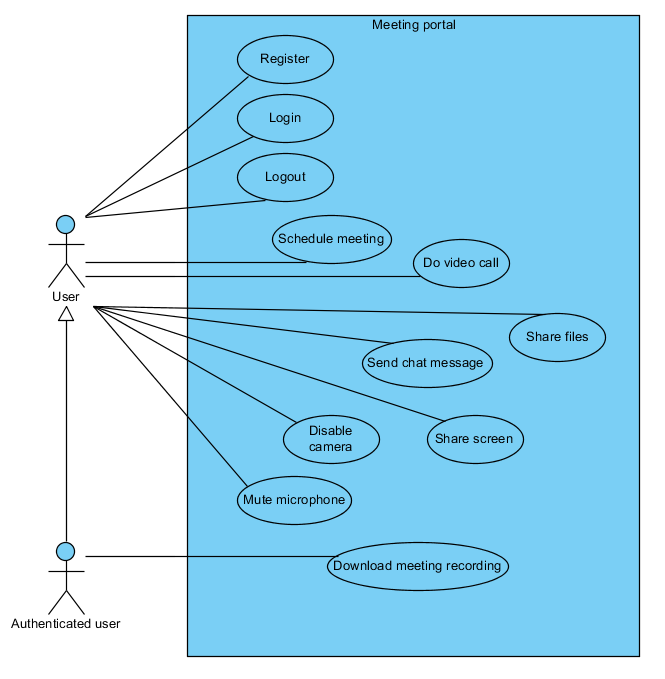
\includegraphics[scale=0.7]{diagrams/use_case.png}
  \end{center}
  \caption{Use case diagram for the portal}
  \label{fig:useCase}
\end{figure}

\section{Nonfunctional requirements}
As the portal is mostly used for communication inside business organization or with its customers, focus should be placed on possibility to connect great number of users together in one call. Teams within organization can be large, so it should be possible to connect several people with reasonable requirements on the network bandwidth of each user. In the context of WebRTC applications this is usually accomplished using the multimedia control units or MCUs for short as mediators of the call.

The portal should also be secure, so all communication is made via secure protocols like HTTPS, or WSS. When the call is made between the members of the organization they have to login using their accounts which they created beforehand. 

All features should be available without the need for the users to install any third-party software. This third-party software includes browser plugins, extensions or any other desktop application. This limitation does not include screen sharing because as of the time of writing this thesis there is no standardized native way for the browsers to obtain the recording of the user's screen. For example, for the chrome browser there is need to install extension\footnote{WebRTC Desktop Sharing - https://chrome.google.com/webstore/detail/webrtc-desktop-sharing/nkemblooioekjnpfekmjhpgkackcajhg} to be able to do screen sharing.

\chapter{Technologies}
This chapter is concerned with introducing the core technologies used for the implementation of the portal. Because software development is not only about languages used but the tools used during the development are equally important it also describes some of those tools.

\section{WebRTC}
WebRTC is an industry and standards effort to put real-time communications capabilities into all browsers and make these capabilities accessible to web developers via standard HTML5 tags and Javascript API\footnote{Application Programming Interface}s \cite{webrtcBook}.

It provides APIs for making audio and video calls directly in the browser. It also contains APIs for file transfer. All the provided APIs are based on peer-to-peer communication, so the data are transferred directly between clients without the need to transfer them to intermediary server. The server is only responsible for establishing the initial connection. This is done via process called signaling. During this process participants exchange meta data about their capabilities. WebRTC does not enforce any particular protocol for signaling and therefore any already existing protocol can be used. Most commonly used protocols include XMPP\footnote{Extensible Messaging and Presence Protocol} and SIP\footnote{Session Initiation Protocol}. 

However, when multiple users participate in a call, peer-to-peer architecture does not scale well. Each peer must upload its stream to every other participant, creating huge requirements on the upload bandwidth. It is possible to route the communication through central server called MCU -- Multimedia Control Unit, which can be responsible for processing the incoming streams and forwarding them to the other participants. Therefore, the peer can send the stream only to this server, reducing the requirements on the connection speeds.

\section{React}
React is a Javascript framework used for building client applications on the web. React was originally created by engineers at Facebook to solve the challenges involved when developing complex user interfaces with datasets that change over time \cite{react}.

React is based on declarative view in which you describe how the view should look based on the data it has available. When the data changes it triggers re-render of all the affected views. It allows to split the views into smaller, encapsulated components. Each component is then responsible for its own rendering based on the provided data. Components can be declared using custom language called JSX, which has similar syntax to HTML, or by using plain Javascript. 

The components can be divided into two categories. Simple components do not contain any logic and are only responsible for rendering the data. On the other hand, there are stateful components which can contain and manage their own state. When this internal state changes the component and all of it children component will be updated based on this new data.

\section{Version control}
Almost no software project today is written without any kind of version control system or also called source control management tool. Version control is a system that records changes to a file or set of files over time so that you can recall specific versions later \cite{proGit}. Most popular version control systems are Git\footnote{https://git-scm.com/}, Subversion\footnote{https://subversion.apache.org/} and Mercurial\footnote{https://www.mercurial-scm.org/}.

For the purposes of this thesis Git was selected as version control system of choice. Git is a distributed version control system which means that the entire history of the repository is kept on the server and on each computer, that creates a clone of the repository from the server. This is a huge advantage in case one of the computers fails. In such scenario nothing is lost because the repository is also kept on other computers and the one which failed can be restored from these clones.

The code is hosted on GitHub which is a cloud hosting platform for Git repositories. It has many features for the project management and source hosting. Some of its most popular features include tools for code review, issue tracking, documentation and team management. It is also very easy to integrate other tools, such as continuous integration servers, with GitHub.

\section{Continuous integration}
Continuous integration is a practice of frequently integrating software components together into the central repository. After this integration automated builds are run to verify that the changes that are being integrated into the base did not break anything and that the system can still be built properly without any errors. A build may consist of the compilation, testing, inspection, and deployment -- among other things \cite{ci}.

It involves having the code repository accessible for a server on which runs an automation component called build service. This build service is monitoring the repository for changes and when any changes occur it triggers the run of predefined jobs on the repository to verify its status. Most popular tools for continuous integration include Jenkins\footnote{https://jenkins-ci.org}, Travis CI, TeamCity\footnote{https://jetbrains.com/teamcity}, Bamboo\footnote{https://www.atlassian.com/software/bamboo} and many others.

For the purposes of this thesis Travis CI was selected as it does not require installation on premises and can easily be configured to work with GitHub. It is free for public open source projects hosted on GitHub.

\chapter{Architecture}
Here will be described the architecture of the portal.

\chapter{Deployment}
Description of how the portal can be deployed will follow here.

\chapter{Implementation evaluation}
Here will be technical evaluation of the portal implementation.

\chapter{Business evaluation}
Business evaluation of the portal. Requirements, how much can it cost to run it on premises, ...

\chapter{Conclusion}

\printbibliography[heading=bibintoc] %% Print the bibliography.

\appendix %% Start the appendices.
\chapter{An appendix}
The source code for the portal is available in the archive in the Information System of Masaryk University.

\end{document}
